\vspace*{4cm}

\begin{figure}[H]
	
\includegraphics[width=4cm, left]{figures/upper-quote-marks.png}
\end{figure}

\textit{$"$In der Welt der drahtlosen Kommunikation sind Antennen die Stimme, die ohne Worte spricht, aber dennoch eine universelle Sprache vermittelt."} \\
\newline
\rightline{Unbekannt} \\
\vspace{2cm}
\newline
\textit{"Von Anfang an übertraf Maxwells Theorie alle anderen an Eleganz und an der Vielzahl der Beziehungen zwischen den verschiedenen Phänomenen, die sie einschloss."}\\
\newline
\rightline{Heinrich Hertz}
\vspace{1cm}

\begin{figure}[H]
	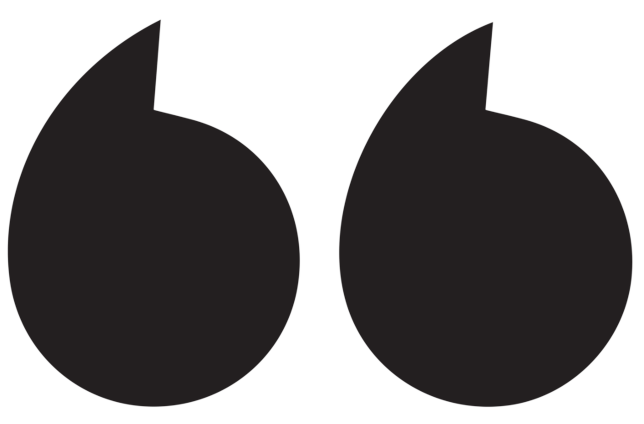
\includegraphics[width=4cm, right]{figures/lower-quote-marks.png}
\end{figure}




